\chapter{Background: Electrical Power System  \label{cha:chapter2}}
This section is intended to provide essential knowledge on EPS that will help to explain the development of PDU.
 

\section{Electrircal Power System Overview \label{sec:tech}}
The EPS is a vital part of a CubeSat-bus. It is responsible for the power generation, energy storage, the processing of electrical power to a defined state and the power distribution across all satellite subsystems. The EPS accounts for a 3rd of the spacecraft mass and is a core subsystem. Power generation technology combine a solar cells, charger. Power storage typically includes a batteries; primary batteries (non-rechargeable), or secondary batteries (rechargeable). Power distribution consist of power switchers, which facilitate power control to a subsystems of the spacecraft.

Fig. \ref{fig: EPSS} illustrates an example of the EPS block diagram.



	\begin{figure}[h]
		\centering
		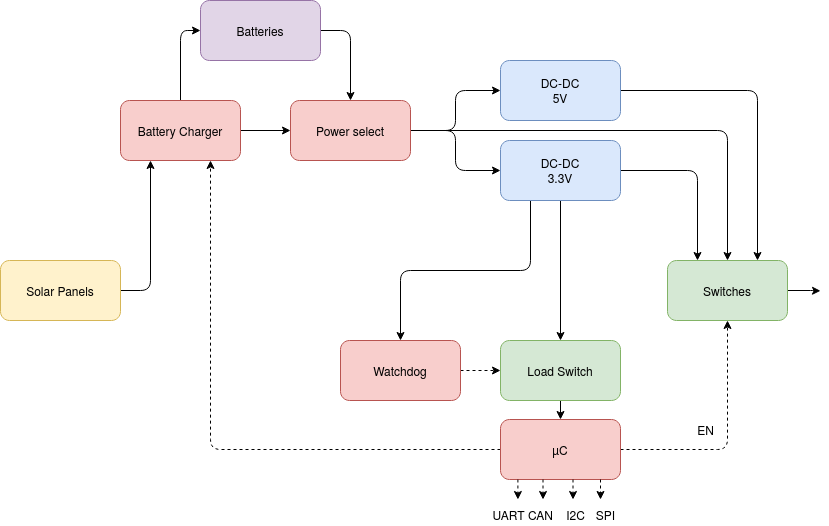
\includegraphics[scale=0.4]{EPS_basic.png}
			\caption{Example of the EPS Block Diagram}
			\label{fig: EPSS}
	\end{figure}

\subsection{Power Generation \label{sec:tech}}



Yost\cite{1} Solar power generation is the most used method for the nanosatellites to generate a power. Solar cells are build of thin silicon disks (semiconductor wafers)  which convert the energy of a light into electric current. Solar intensity of a solar array is light availability of the sun, which can vary according to a distance from the sun as well as angle of a projected surface area between the sun and a solar array.  
\\
\noindent\hspace*{3mm} Alia-Novobilski\cite{2} The most common manufactured type of cells are single junction cells. Single junction type is commonly used on the Earth applications. Due to severe sensitivity to a space radiation energy and relatively low efficiency, single junction type is not preferable for a space applications. Although single junction solar cell is relatively cheap to design, modern spacecraft use a multi-junction solar cells. Manufactured of a light-absorbing materials, multiple layers are much tolerant to a radiation in a space environment and more efficiently  Yost\cite{1} "convert specific wavelength regions of the solar spectrum into energy, thereby using a wider spectrum of solar radiation ". 
Green\cite{3} In the space industry, triple-junction solar cells are the most common tu use due to their high efficiency and relatively affordable cost compared to an other types of solar cells.

Fig. \ref{fig: GaAs} illustrates the example of a Triple Junction GaAs Solar Cell.

\begin{figure}[h]
	\centering
	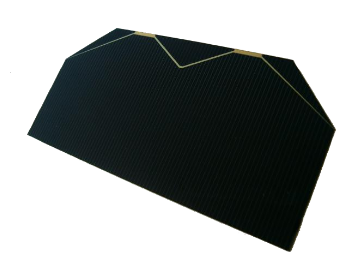
\includegraphics[scale=0.4]{azur.png}
	\caption{ 30\% Triple Junction GaAs Solar Cell \cite{4}}
	\label{fig: GaAs}
\end{figure}

Solar cells are usually interconnected to a solar array to get the desired power. Configuration of the solar array is flexible, such that it allows adjustment of the cells connection. To achieve the desired voltage, solar cells get interconnected in series (strings). To achieve the desired current, solar cells get interconnected in parallel.\\

\newpage

\begin{figure}[h]
	\centering
	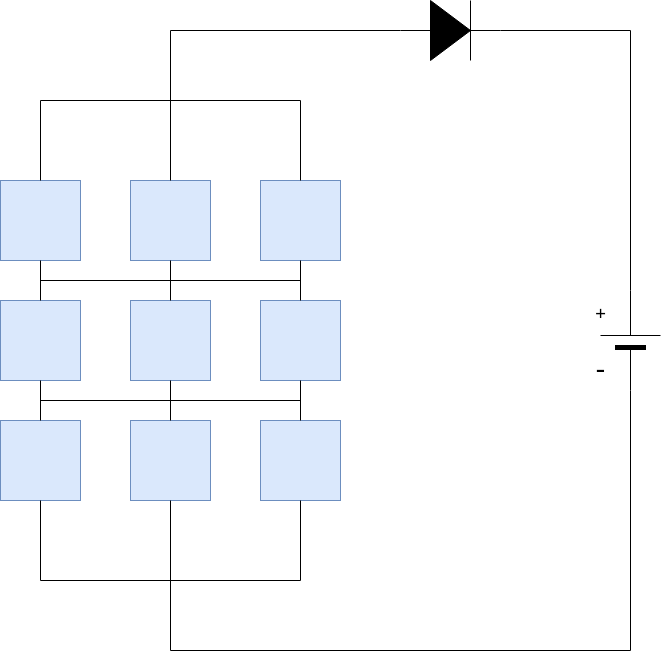
\includegraphics[scale=0.3]{Cellen.png}
	\caption{ Solar array}
	\label{array}
\end{figure}
	
Solar cell is strongly effected by a temperature. Honsberg\cite{5} "Increases in temperature reduce the band gap of a semiconductor, thereby effecting most of the semiconductor material parameters. The decrease in the band gap of a semiconductor with increasing temperature can be viewed as increasing the energy of the electrons in the material."\\
\\
Brieß\cite{6} The dependency of a temperature to the electric power of a silicon solar cell can be described as:\\ \\ \\

\begin{equation}
P = P_{ref} [ 1 - K_{P} ( T - T_{ref}) ]
\end{equation}
	\\
	\\
where:\\
     $P_{ref}$ - Power at reference temperature\\
     $K_{P}$ - Correction factor of power losses, 0.005$K^{-1}(for a silicon solar cell)$\\
     $T_{ref}$ - Reference temperature ( e.g. 25\textdegree{}C)\\
     
     

\begin{multicols}{2}
	\textbf{High  temperature:} \\ \\
	$\bullet$ reduce cell voltage \\
	$\bullet$ increase a cell current\\
	$\bullet$ reduce power\\
	

	\columnbreak
	
	\textbf{Low temperature:}\\ \\
	$\bullet$ increase cell voltage\\
	$\bullet$ reduce a cell current\\
	$\bullet$ increase power\\
	\\
\end{multicols}


	\begin{figure}[h]
		\centering
		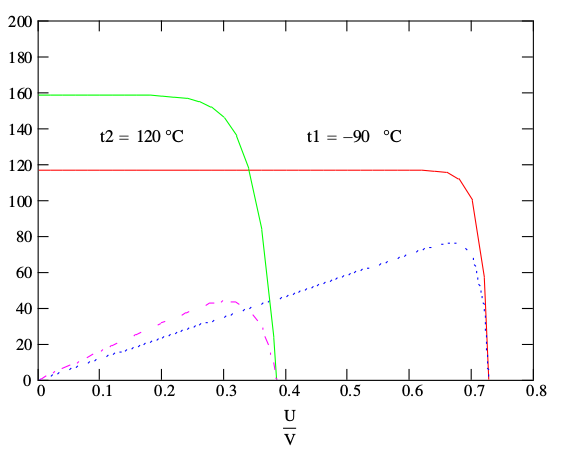
\includegraphics[scale=0.5]{temperatureDependancy.png}
		\caption{ Example of a solar cell characteristics at different temperatures\cite{6} }
		\label{fig: EPS11}
	\end{figure}
	
According to a Fig. \ref{fig: EPS11} a maximum power point shifts as a solar array getting hotter or colder. To keep power at the maximum point used Maximum Power Point Tracker (MPPT). The purpose of MPPT is to keep voltage on a particular level while solar panels are affected by a temperature or the orientation of the solar panels.\\
\cite{20} MPPT might be separated into two parts: power control, logic control. Power control is usually a step-up step-down DC-DC  converter which responsible for a voltage adjustment according to the input from the logic control. Logic control is responsible for a solar array parameters measurements and maximum power point adjustment according to the software algorithm.\\  

During the circuit design of the solar panels, it is important to consider the redundancy and a case in which one of the cells will be damaged. For that reason diodes are used. The diodes ensure the power can bypass a damage solar cell. Fig. \ref{dioden} illustrates the diodes D1 and D2 which are placed in the parallel with the solar cells. The diode D3 which can be also observed on the Fig. \ref{array} is used to prevent the reverse current. Reverse current has a negative effect on the solar panel efficiency. When reverse current occurs, it begins to draw current from the batteries, hence discharging them. In addition, reversed current adds additional current to the affected solar cell which shifts the maximum power point.\\


\begin{figure}[h]
	\centering
	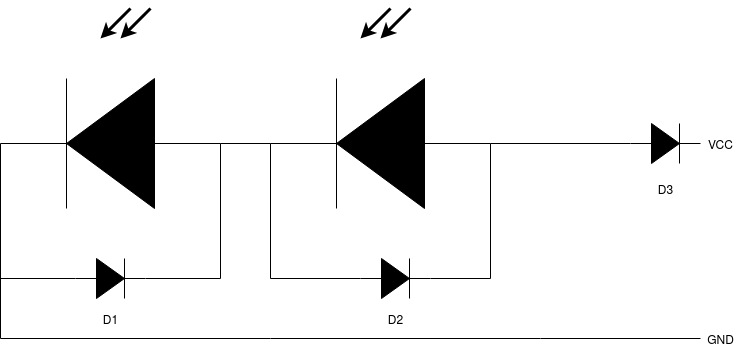
\includegraphics[scale=0.45]{DiodenSS.png}
	\caption{ Example of the Solar cell circuit design}
	\label{dioden}
\end{figure}
 
\newpage


\subsection{Power Storage \label{sec:tech1}}



Yost\cite{1} During the the mission duration, solar energy is not always available due to eclipse. For this case primary and secondary batteries used to store power. All batteries are classified according to their chemical characteristics. For a short mission duration (up to one week)  the primary type of batteries are usually used due to the lack of the possibility of recharging. The common chemical type of a primary battery is a silver-zinc, which is easier to handle, Yost\cite{1} "however there is also a variety of lithium-based primary batteries that have a higher energy density including: lithium sulphur dioxide (LiSO2), lithium carbon monofluoride (LiCFx) and lithium thionyl chloride (LiSOCl2)."\\
\\
Secondary-type batteries are rechargeable and provide an energy on demand. Secondary-type batteries are connected to a primary energy source of the satellite (usually solar panels) via battery charger. This type include: nickel-cadmium (NiCd), nickel-hydrogen (NiH2), lithium-ion polymer(LiPo), lithium-ion(Li-ion).

\subsubsection{Nickel Cadmium \label{sec:tech}}
 Buchmann\cite{7} Nickel Cadmium is a type of rechargeable batteries using nickel oxide hydroxide and metallic cadmium. This chemical connection allows battery to well perform by working in the savage conditions such as low or hot temperature. NiCd battery is the type which prefer to be charge fast instead of slow as types of secondary batteries. Full periodic discharge of a NiCd is an important process and necessary for battery performance. In case of absence  Buchmann\cite{7} " large crystals will form on the cell plates (also referred to as memory) and the NiCd will gradually lose its performance."
 
 \newpage

\begin{multicols}{2}

	\textbf{Advantages:} \\ \\
	$\bullet$ Big variety of size and performance options\\
	$\bullet$ Low price\\
	$\bullet$ One of the most robust rechargeable batteries\\
	$\bullet$ Good performance in the low temperature\\
	$\bullet$ Simple and fast charge\\
	$\bullet$ Big number of discharge cycles\\
	
	
	\columnbreak
	
	\textbf{Disadvantages:} \\ \\
	$\bullet$ Low energy density\\
	$\bullet$ NiCd has to be periodically discharged\\
	$\bullet$ NiCd contains toxic metals\\ 


\end{multicols}

Fig. \ref{fig: nicd} illustrates an example of the NiCd battery. 



\begin{figure}[h]
	\centering
	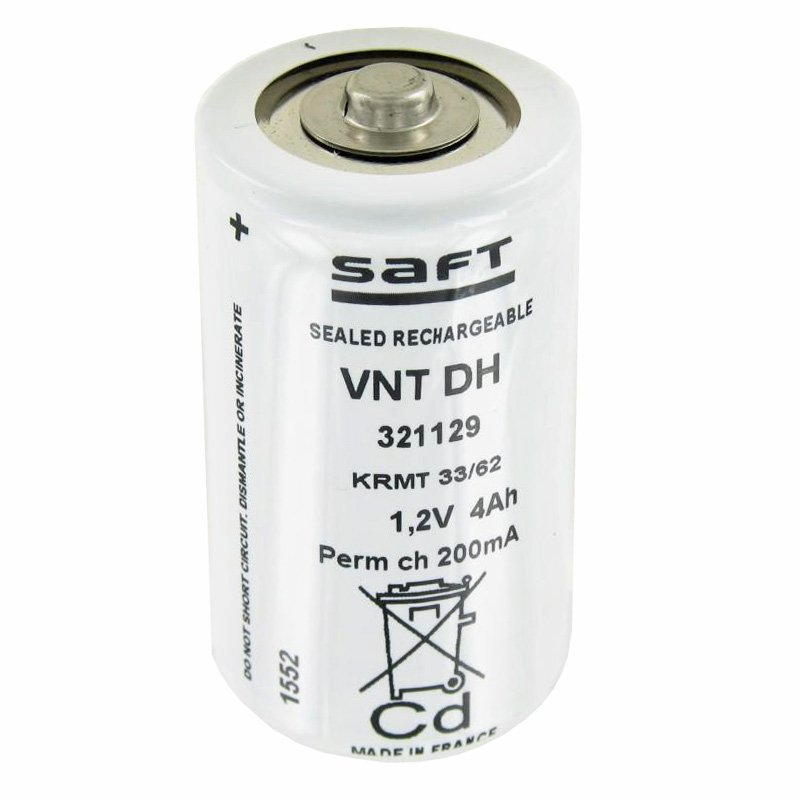
\includegraphics[scale=0.1]{NiCd.jpg}
	\caption{NiCd battery\cite{9}}
	\label{fig: nicd}
\end{figure} 


\subsubsection{Nickel Hydrogen \label{sec:tech}}
Buchmann\cite{7} Nowadays Nickel Hydrogen batteries are mostly used in the satellite applications where long time operation is required. The development of the NiH2 battery started in early 1970 year. In that time metal hybrid alloy was unstable, what slowed down development of the NiH2. In 1980 new alloy was established and stable enough to use it in the cell. 
\cite{10}"The replacement of cadmium with hydrogen electrodes has double the energy of Ni-Cd, but the specific energy of Ni- H2 is similar to Ni-Cd be case of the cylindrical configuration of the pressure. The first Ni- H2 battery was used in a GEO (geostationary mission) Intelsat V in 1983.  Almost all GEO spacecrafts now use Ni-H2 batteries. The first NASA LEO spacecraft to use Ni-H2 was in 1990."


Wenige\cite{8} Despite the fact that memory effect on NiH2 is undoubtedly less than on a NiCd batteries, it still exist and needs a special treatment in order to accommodate the normal level of the battery. Wenige\cite{8} "Typical calendar life of more than 20 years can be reached by NiH2, i.e. five years ground storage plus 15  years  orbital  life  in  GEO." \\ \\


\begin{multicols}{2}
	
	\textbf{Advantages:} \\ \\
	$\bullet$ High energy density\\
	$\bullet$ Environmentally friendly\\
	$\bullet$ Cheap\\
	$\bullet$ Less prone to memory effect\\
	$\bullet$ Suitable for a long life Satellite missions\\
	

	
	
	\columnbreak
	
	\textbf{Disadvantages:} \\ \\
	$\bullet$ Lose performance after deep discharge with high load\\
	$\bullet$ Requires long charge time due to heat generation\\
	$\bullet$ Require regular discharge to prevent memory effect\\ 
	$\bullet$ More expensive than a NiCd\\
	$\bullet$ Long life cycle

	
\end{multicols}

Fig. \ref{fig: nih2} illustrates an example of the NiH2 battery. 


\begin{figure}[h]
	\centering
	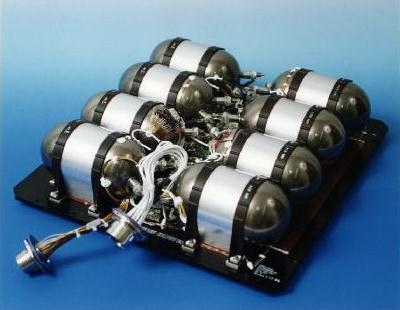
\includegraphics[scale=0.3]{NiH2.jpg}
	\caption{ NiH2 battery \cite{10}}
	\label{fig: nih2}
\end{figure}

\subsubsection{Lithium Ion \label{sec:tech}}

Buchmann\cite{7}Today lithium ion batteries is the most progressive and most promising batteries. Lithium is the lightest metal and able to provide the biggest energy density per weight. The energy density of a Lithium Ion batteries is about two times bigger then a NiCd. In addition, discharge characteristics of a Li-ion are similar to a NiCd, which offers a save utilization of a Li-ion batteries. Another advantage of a Li-ion batteries is a high cell voltage, which allows to allows to keep power properties with the light mass. Despite the fact that Li-ion batteries have many advantages, they also have their drawbacks. Li-ion batteries are very sensitive to an overcharge as well as an over discharge. For that reason Li-ion batteries usually used with protection circuits, which limit the peak voltage. In addition Li-ion batteries are prone to age even if not used Buchmann\cite{7} Over two or perhaps three years, the battery frequently fails.


\begin{multicols}{2}
	
	\textbf{Advantages:} \\ \\
	$\bullet$ High energy density\\
	$\bullet$ Low self discharge\\
	$\bullet$ No memory\\
	$\bullet$ High cell voltage\\
	
	
	
	
	\columnbreak
	
	\textbf{Disadvantages:} \\ \\
	$\bullet$ Require protection circuit\\
	$\bullet$ Aging without using\\
	$\bullet$ Does not apply for a long term use\\
	$\bullet$ Proper storage needed 

	
	
\end{multicols}

Fig. \ref{fig: lion} illustrates an example of the Li-ion battery. 

\begin{figure}[h]
	\centering
	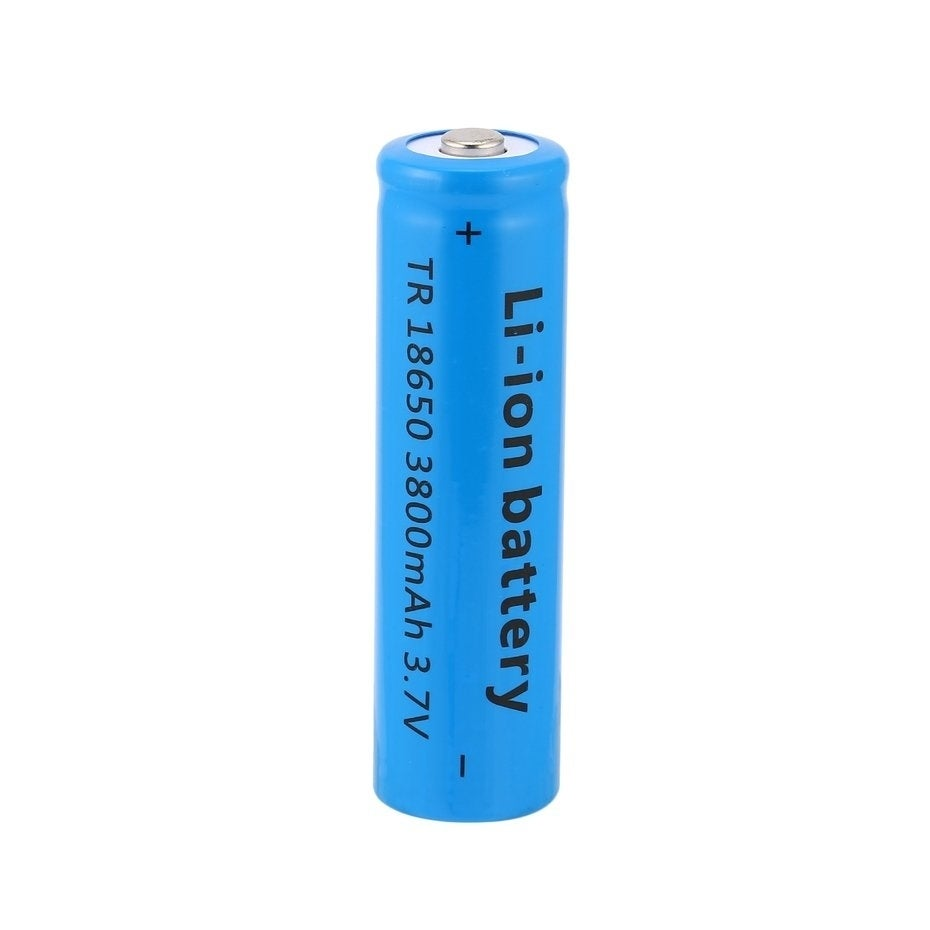
\includegraphics[scale=0.11 ]{Li-ion.jpg}
	\caption{ Li-ion battery \cite{11}}
	\label{fig: lion}
\end{figure}

\subsubsection{Lithium Polymer \label{sec:tech}}

In 1970, when the original design of lithium polymer batteries was invented, dry solid polymer electrolyte was used instead of  porous separator. Dry polymer design, allows to simplify manufacture process and the most important - to have a thin thickness geometry. However Dry solid polymer electrolyte experienced poor conductivity due to internal resistance of a the battery. Thereby, gelled electrolyte has been added to enhance ion conductivity. LiPo batteries have a slightly lower energy density and amount of charge/discharge cycles compare to Li-ion batteries. Nonetheless LiPo batteries have a bigger overcharge tolerance, which making them more robust to overcharge conditions.


\begin{multicols}{2}
	
	\textbf{Advantages:} \\ \\
	$\bullet$ Low profile \\
	$\bullet$ Flexibility to produce any shape\\
	$\bullet$ Weight\\
	$\bullet$ Resistant to overcharge\\
	
	
	
	
	\columnbreak
	
	\textbf{Disadvantages:} \\ \\
	$\bullet$ Lower energy density\\
	$\bullet$ Expensive\\
	$\bullet$ Does not apply for a long term use\\
	$\bullet$ Proper storage needed 
	
	
	
\end{multicols}

Fig. \ref{fig: lipo} illustrates an example of the LiPo battery. 

\begin{figure}[h]
	\centering
	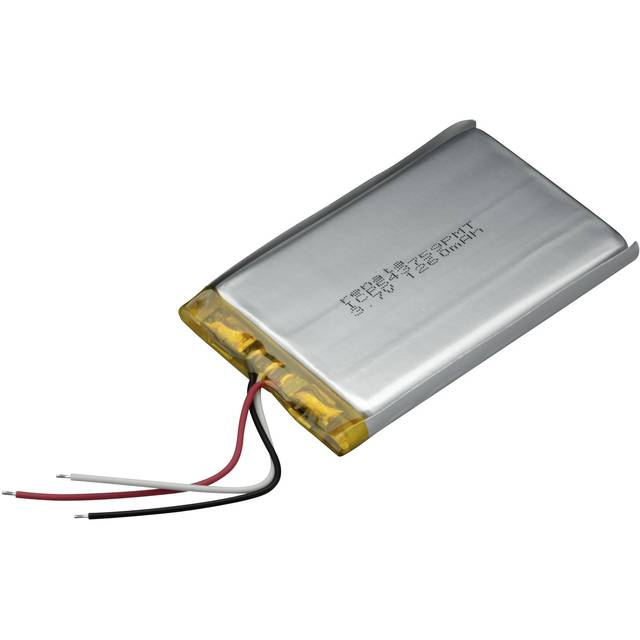
\includegraphics[scale=0.16]{LiPo.jpg}
	\caption{ LiPo battery \cite{12}}
	\label{fig: lipo}
\end{figure}



\subsubsection{Charging}

Santoni\cite{13}The hight capacity and low weight make Li-ion batteries very well suited for a nanosatellite space applications. Nonetheless performance and safety charging issues should be taking into account. Insidor\cite{14} The charge of a LI-ion batteries is very strict on the correct settings, mostly due to a high sensitivity to a overcharge. Typical Li-ion battery voltage per cell can vary from 4.1 to 4.3, which is defined in the datasheet. However, typical and most common value is 4.2V. Exceed of a battery voltage limit will increase capacity, but will also stress a battery, which can seriously harm a cell and and significantly reduce battery performances.\\ \\
Li-ion/Po battery charge process can be divided into 2 main stages:\\
$\bullet$ constant current charge\\
$\bullet$ constant voltage charge\\

Fig. \ref{fig: bcs} illustrates the example of battery charging stages.

\begin{figure}[h]
	\centering
	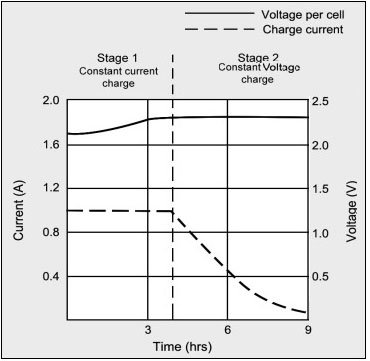
\includegraphics[scale=0.7]{bcs.jpg}
	\caption{ Charge stages \cite{14}}
	\label{fig: bcs}
\end{figure}
 Charging rate of a battery measures in C. In case of 1000mAh battery cell 1C charging rate will be 1000mA and 500mA for 0.5C. Usually, recommended charging given in the datasheet.\\
 Charging process starts with a 100\%  constant current (according to a charging rate) process. During the time while battery voltage reaching the upper voltage threshold, its pushing a constant current into a battery. Once voltage reaches threshold point, charging process changes from the constant current mode into a constant voltage mode. In a constant voltage mode, voltage keeps its maximum level while current starts to slightly drop until it gets down to a threshold level, which usually written in a datasheet (around 3\%). After current drops below the threshold, battery is fully charged. \\ \\
 In most cases, IC chargers are used to provide constant current and constant voltage for lithium-ion / Po batteries. \cite{14} One of those IC chargers is a MAX745. 
This IC is able to set a charge up to 4 cells in series, as well as set a current and charging voltage. This IC use PWM signal to control a charge voltage which does not allow IC to get too hot.\\ This IC is an example of a charger microchip which has all necessary  tools to charge a Li-ion/Po batteries. 



\begin{figure}[h]
	\centering
	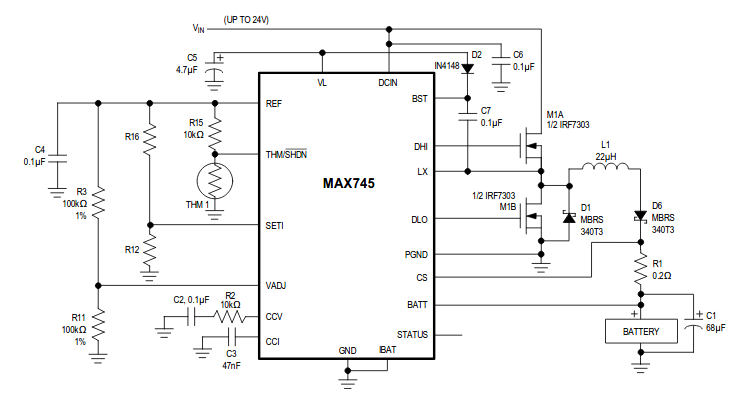
\includegraphics[scale=0.5]{MAX745.png}
	\caption{ Li-ion/Po charger MAX745 \cite{15}}
	\label{fig: EPS22}
\end{figure}

The Figure \ref{fig: EPS22} shows an example of a standard MAX745 application circuit. On the left side of the schematics pins SETI and VADJ are used to adjust a charge voltage and charge current. External resistors R16,R12 are connected to a reference voltage to adjust a charge current and resistors R3,R11  used to adjust charge voltage. On the right side of the schematics MAX745 use two external N-channel MOSFETs which control power from the input source which controlled by current mode, PWM controller. 



\subsubsection{Protection}

Despite the fact that, Lithium-ion/Po batteries have a high density, they also require a careful handling. For this reason, it is important to use protective circuits that prevent overcharging, over-discharge and quick discharge of Li-ion batteries.\\
\cite{16} Overcharge of a Li-ion/Po batteries case an immense battery stress which creates a safety hazard with a possibility of fire. Li-ion batteries have a less tolerance to an overcharge and require a protection circuit.\\
The over-discharge of a Lithium batteries is also harmful. The consequence of over-discharge is a reduced battery life, due to the dissolution of copper from the anode into the electrolyte, which can case a short circuit during a battery charge.\\
Protection ICs used to comply all upper mention conditions. A main principal of a protection IC is to switch on and off a power line usually by using external MOSFETs to keep a batteries safe and not exceed a voltage threshold. The simple example of a protection IC is a BQ29700D which is a one cell protection device. 

\begin{figure}[h]
	\centering
	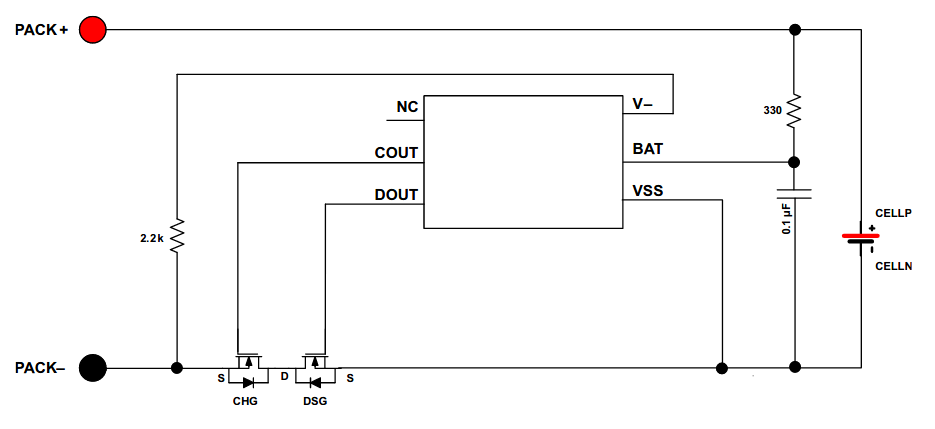
\includegraphics[scale=0.5]{protect.png}
	\caption{ BQ29700D protection IC \cite{17}}
	\label{fig: EPS1}
\end{figure}

Figure \ref{fig: EPS1} illustrate a typical schematics of a protection circuit where BQ29700 connected with two MOSFETs defined as CHG and DSG, and a battery cell. In case of overcharge detection, COUT pin pulls a CHG MOSFET which disconnect ground line and stops charging process. In case ocer-discharge detection, DOUT pin pulls a DSG MOSFET which dissconect ground line and stops discharging process of a battery.

\subsection{Power processing \label{sec:tech}}

Power processing is an important part of an EPS which is responsible for transforming voltages to be suitable for satellite subsystems and payloads. Nowadays there are many converters available; each type has it's own advantages and disadvantages. Hemmo\cite{18} A converter has to be chosen according to subsystem requirements such as voltage range, maximum power output, output voltage tolerance, efficiency and footprint. The power efficiency of a converter is a very important criterion of stored energy due to the fact that battery energy is limited. High efficiency of  power conversion reduces the power dissipation of  components, thereby decreasing the power consumption if batteries. Furthermore, the need for any heat sinks is reduced or altogether eliminated. 

\subsubsection{Linear Voltage Converters \label{sec:tech}}

Hemmo\cite{18} One of the oldest methods to convert a power is a linear voltage conversion. This method based on power dissipation into a resistor, which case a voltage drop. Power dissipation of a linear voltage converter can be calculated by using formula:\\ \\

\begin{equation}\label{eq:2}
P_{diss}=U_{drop} \times I
\end{equation}


where:\\
$U_{drop}$ - resistor voltage drop\\
$I$ - current through a resisor\\ \\
 Tietze \cite{18} Linear voltage conversion is a simple method, which does not require many additional passive components, relatively cheap and easy to use. Nonetheless due to a power dissipation linear voltage converters are getting hot, which make them ineffective while current through a resistor is large or difference between $V_{in}$ and $V_{out}$ is high according to \eqref{eq:2}. For that reason Linear voltage converters used only in case of low current and low voltage drop for example to convert power into a micro controller or to provide a voltage reference.\\
 \\
 
 
\subsubsection{Inductive DC-DC Converters \label{sec:tech}}

Tietze\cite{18} Each inductive DC-DC converter consist of three passive components: inductor $L$, power switch $S$ and capacitor $C$. The use of these components in various topologies, allow to create various types of DC-DC converters such as a step-down converter where output voltage $0 \leq U_{a} \leq U_{e} $ , step-up converter where output voltage $U_{a} \geq U_{e} $  and   step-down step-up converter which is able to decrease and increase output voltage, for this type of a converter $ U_{a} > 0$. Use of inductive DC-DC converters offer better efficiency due to switching power supply, which gives an advantage over the linear voltage regulator. Hemmo\cite{17} High efficiency is extremely required parameter for a space application due to the limited power generation. In addition, inductive DC-DC converters are able to produce  voltage output $U_{a}$ which is higher then voltage input $U_{e}$. Inductive DC-DC converters used in most cases in the aerospace industry due to high efficiency and capability to manage high voltages and high current.

\begin{figure}[h]
	\centering
	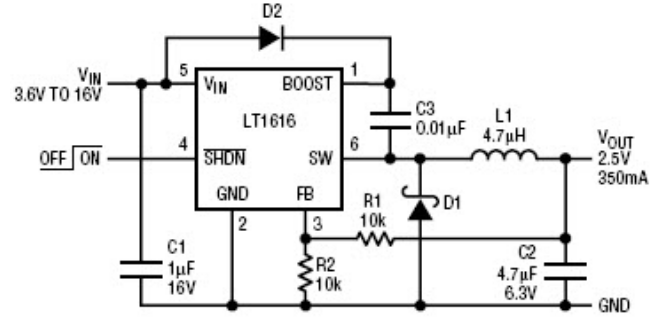
\includegraphics[scale=0.4]{ltc1616.png}
	\caption{ Inductive DC-DC converter \cite{19}}
	\label{fig: EPS41}
\end{figure}

Figure \ref{fig: EPS41} illustrates an example of the simple Inductive DC-DC step-down converter LT1616. The inductor L1 allows peak current to be reduced in order to not harm the C2 capacitor and to store the energy while the inner switch is closed. The diode D1 provide a different path for the current while inner switch of the LT1616 is open. The output voltage of converter can be programmed by choosing a value for the resistors $R1$ and $R2$ according to a formula from the datasheet \cite{19} . 
\\
\\

\subsection{Microcontroller \label{sec:tech}}
The main responsibility of the EPS microcontroller is to manage a power distribution for a hole satellite by sending an enable signals to a commutating components, in most of the cases integrated switches. In addition, microcontroller provide a housekeepeng telemetry by reading the values of sensors, such as temperature sensors, current sensors and others. For this task EPS microcontroller uses protocol lines as $I^{2}C$ or $SPI$. Furthermore, EPS microcontroller needs to communicate to an OBC microcontroller to share the housekeeping information or for reason to receive a commands from OBC. Communication between EPS and OBC as well as with other microcontrollers implemented via CAN bus. Moreover, EPS microcontroller can be used to handle MMPT algorithm to obtain the maximum power from the solar energy. The example of microcontroller block diagram architecture shown on the Fig \ref{fig: EPS4121}.	
\\
\begin{figure}[h]
	\centering
	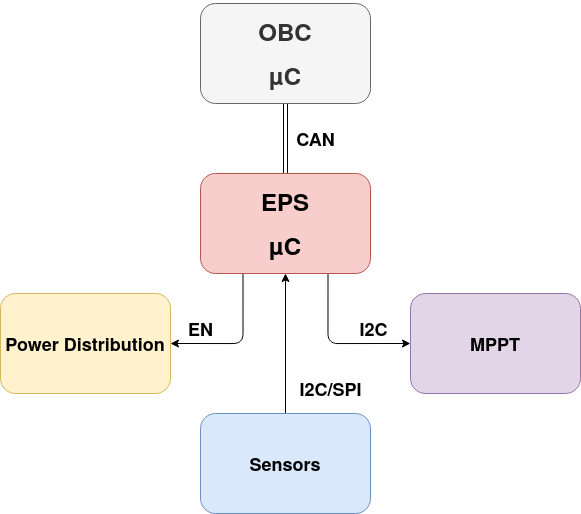
\includegraphics[scale=0.4]{uC.png}
	\caption{block diagram of microcontroller communication}
	\label{fig: EPS4121}
\end{figure}
\\
EPS Data signals:\\ \\
$\bullet$ CAN\\
$\bullet$ UART\\
$\bullet$ I$^{2}$C\\
$\bullet$  SPI\\
$\bullet$  EN\\
\\
As for power consumption, microcontrollers consume very little power. Some microcontrollers such as STM32L  can consume  around 10 to 100 $\mu$A.\\
To prevent the microcontroller of getting stuck, external watchdog is used. Watchdog receives the signal from the microcontroller which restart the timer. If case that watchdog did not receive a signal, he will send a signal to a load switch, which will restart the microcontroller by turning the supply power "OFF" and "ON".

\subsection{Power Distribution \label{sec:tech}}

Power distribution is a vital part of the EPS, needed to \cite{21} "supply electrical power to the subsystems and payloads of the satellite" as well as prevent an overload of the main power bus. Power distribution usually consist of load switches which distribute power with help of microcontroller by sending the enable signal to an appropriate pin of the switch. In addition, current sensors are used to monitor the payload or power consumption of the subsystem. This combination allows to fully control the process of power distribution. Figure \ref{fig: EPS111} illustrates an example of the EPS power distribution where $R_{sense}$ is a shunt resistor for a current sensor. 


\begin{figure}[h]
	\centering
	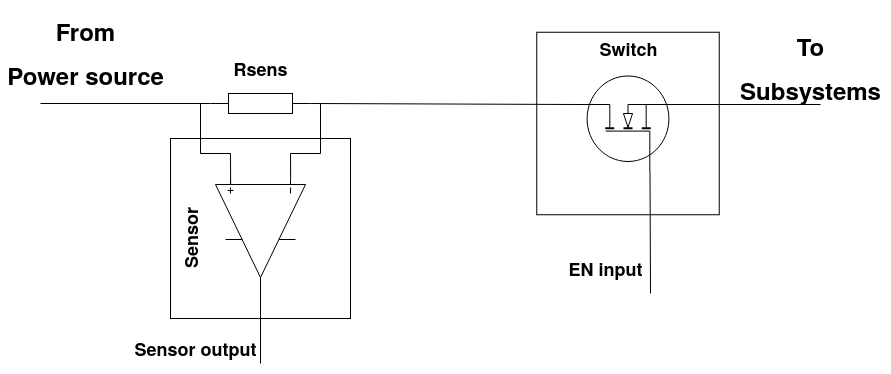
\includegraphics[scale=0.35]{distrib.png}
	\caption{Power distribution with power switch and current sensor}
	\label{fig: EPS111}
\end{figure}

\newpage

\subsubsection{Switches}
Power distribution include load switches which responsible for a power commutation of a satellite. Power switches are integrated chips which designed for specific cases and scenarios. One of the important parameters is a power load. Switches have to be chosen according to a load of a power lines considering voltage and maximum current. Otherwise, if the input power exceeds the power that the switch can operate with, this might lead to destruction of the switch and the entire power line.  Another aspect which has to be considered is the inrush current. Inrush current is a maximal instantaneous current draw by an electrical device, appeared for few microseconds when first turn on. Inrush current cased a voltage drop for the supplied subsystems, which might harm device or case incorrect device performance.

 Capacitors might be used to prevent inrush current. The value of capacitor has to be calculated by equation \ref{eq:3} \cite{32}:
 
 \begin{equation}\label{eq:3}
 C_{L} = I_{INRUSH} \times \dfrac{dt}{dV_{out}}
 \end{equation}
 
 Where:\\ \\
 $I_{INRUSH}$ - amount of inrush current\\
 $C_{L}$ - Value of capacitor \\
 $dV_{out}$ - maximum allowable voltage drop\\
 $dt$ - rise time\\

Another important ability of the switcher is the fault detection. Fault detection appear while current on the power line exceed the programmed current of the switch. Whilst Overcurrent was detected, switch sends a signal to a microcontroller to disable the switch. Fault detection often used to detect Lautch-up of the satellite.\\

\subsubsection{Power Monitoring}

Power monitoring is the necessary part of the EPS, which allows to observe the current status of each subsystem and payloads of the satellite. \cite{22} "Power monitoring is implemented by measuring the 
voltage drop across a shunt resistor.  The voltage across the shunt  is  usually  amplified  using  a  differential amplifier" and produce the analog output. Nowadays Current sensor ICs used to monitor a current on the power lines. Modern current sensors have ability to output measured information as I$^{2}$C or SPI data by converting an analog output signal to the digital via integrated analog to digital converter. 

\newpage   
\chapter{6 Unit Satellite Design \label{chapter3}}
This chapter will provide a short essential knowledge about Descartes Mission with the main purposes of the mission, satellite characteristics and the satellite  abilities. Then topic will go deeper into the EPS architecture design of the 6U satellite. \\
\section{Introduction into the Descartes Mission}

German Orbital System (GOS) plays a major role in the satellite development. GOS has accomplished nine successful 3U satellites launches into space since their realize as a company. Although 3U satellites are relatively cheap to build and their characteristics enough have a simple payload, GOS is keeping up with the time. At the moment GOS is developing the 6U nanosatellite (Descartes), that shown on the Figure \ref{fig: EPS222}. Descartes can be used for a wide range of tasks such as:\\ \\
$\bullet$ Earth exploration\\ 
$\bullet$ Student projects\\ 
$\bullet$ Science projects\\ 
$\bullet$ Orbit calibration and control\\ 
$\bullet$ Auto Dependent Surveillance Broadcast\\ 



\begin{figure}[h]
	\centering
	\includegraphics[scale=0.19, angle =90]{descart.png}
	\caption{The Descartes satellite}
	\label{fig: EPS222}
\end{figure}


  Descartes is a 6U satellite with dimensions 360$\times$240$\times$120 and mass less than 8kg. 6U satellite has 3.5U of payload free space, which is reserved for the four different payloads. Descartes developed for a 2 years of lifetime on the Low Earth Orbit. For his orbital lifetime satellite will measure the space weather, observe the aircrafts, monitor the ultraviolet radiation on the Earth atmosphere  and provide remote sensing of Earth. The Space weather measurements implemented by DeCor payload. DeCor is a detector of gamma radiation and charged particles in the range of 0.3-3 MeV.This device allows to study the fast variations of electron fluxes in the gap zone between radiation belts and dynamics of particle fluxes and gamma radiation in low orbits depending on geomagnetic conditions. Aircraft data are monitored using a payload called AMUR. AMUR is designed to collect, process and filter aircraft data. 
  In addition to having a four different payloads, Descartes is using 3-axis attitude control which consist of reaction wheels, magnetorquers and sets of magnetic and solar sensors. To transmit the telemetry and commands Descartes use 2 UHF modules which were designed ba GOS. In addition to 2 UHF modules, 6U satellite operate with a 2.4 GHz HISPICO S-band transceiver.\\ \\
 
 
  \section{EPS Architecture of the 6U Satellite}
  According to an introduction into the mission it is noticeable that design of the 6U satellite highly improved in comparison with the previous 3U satellites which were designed by GOS. The biggest divergence is a size and availability of the satellite to work with more payloads as well as to perform 3-axis stabilization. Due to that fact, the EPS of the satellite has also undergone changes.
  
  Due to the energy requirements, 6U satellite has to provide a 160 Wh of energy and  distribute it to 23 channels. To accomplish this requirements, considering the available space of the 6U satellite, EPS was devided into 3 main parts which connectrd between each other via PC104 connector:\\ \\
  $\bullet$ Power Proccessing Unit\\
  $\bullet$ Power Distribution Unit\\
  $\bullet$ 2 Battery Packs\\
  
   \subsection{Power Processing Unit}
   PPU is a part of EPS which responsible for a battery charge, power distribution control and a power processing. The PPU is illustrated on the Fig. \ref{fig: psu122}.
   
   \begin{figure}[h]
   	\centering
   	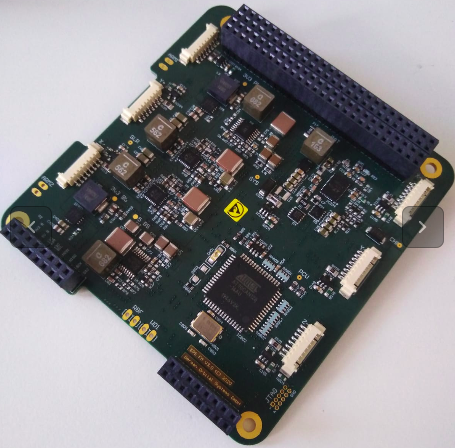
\includegraphics[scale=0.4]{ppu.png}
   	\caption{PPU}
   	\label{fig: psu122}
   \end{figure}
   
   Power converted from the solar flux come first into a PPU from 6 solar panels: X+, X-, Y+, Y-, Z+, Z-. At first, input power of each solar panels gets measured by MAX7328 current sensor. Then power goes into a microchip LTC4015 which is responsiable for a battery charge, illustrated on the Figure \ref{fig: ltc40151}. Integrated circuit LTC4015 provide a constant voltage and current into a batteries at the same time passing unregulated power from the solar panels directly into a system load. Although LTC4015 can be adjusted for a battery charge manually, microchip might use an MPPT algorithm to regulate the voltage in order to keep maximum power peak. This allows to charge and discharge the batteries according to a batteries state of charge and solar condition (eclipse). Microchip draws power from the solar input to the system, while batteries are charging and switch power source to a battery pack while eclipse or overcharge condition.
   
  \begin{figure}[h]
  	\centering
  	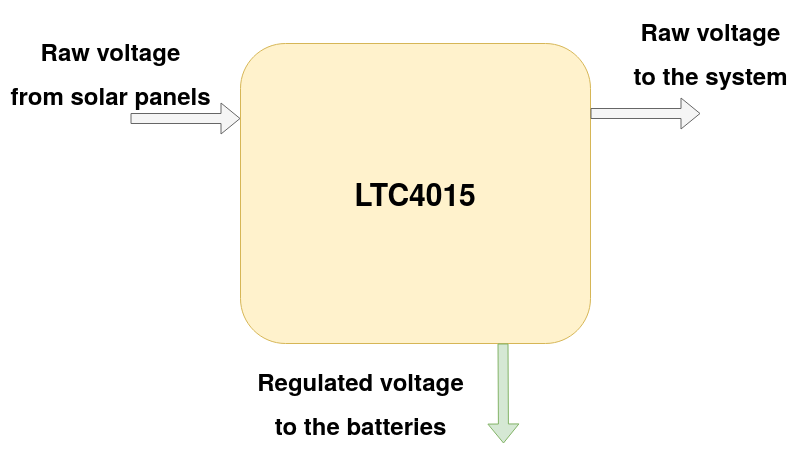
\includegraphics[scale=0.2]{ltc4015.png}
  	\caption{Battery charger}
  	\label{fig: ltc40151}
  \end{figure}
  
 After the power has been distributed from the charger, is separates in two power lines, one power line goes through the LDO converter to feed the microcontroller and second distributes the power into five DC-DC converters for the subsystems and payloads.
 
 LDO converts input power from the charger into 3.3V to supply a power for microcontroller. After surpassing the LDO, power goes through the load switch, controlled by watchdog. Watchdog provide a constant output signal to the load switch, that alloud him to commutate and transfer power further to the microcontroller. 
  
    \begin{figure}[h]
    	\centering
    	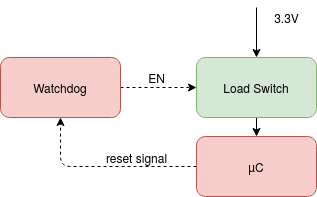
\includegraphics[scale=0.7]{Watch.png}
    	\caption{microcontroler power supply}
    	\label{fig: ltc4015}
    \end{figure}
  Microcontroller sends a reset signal to the watchdog, to to reset the counter. As long as counter reset, watchdog keep the enable output pin "HIGH". However, when watchdog does not receive the reset signal from the microcontroller due to some system problems, watchdog restart himself and enable output pin getting low and high, which restart microcontroller.
  
  5 DC-DC converters of the PPU convert the input power from the LTC4015 charger. Power processing can be divided into 2 blocks power processing for the BUS and power processing for the payload. Each block has 2 DC-DC step down converters, 5V, 3.3V and one common 7.4V. Common 7.4 V converter used to convert unregulated voltage from the solar panels. For this task LTC3119 used, this microchip has a big current tolerance which allows him to transfer huge amount of power.To produce 5V and 3.3V, used LM43603 and TPS62111 converters. This converters were successfully used on the previous EPS models. In order to keep a flight heritage, were made decision to keep the converters as it is. 
  
   \begin{figure}[h]
   	\centering
   	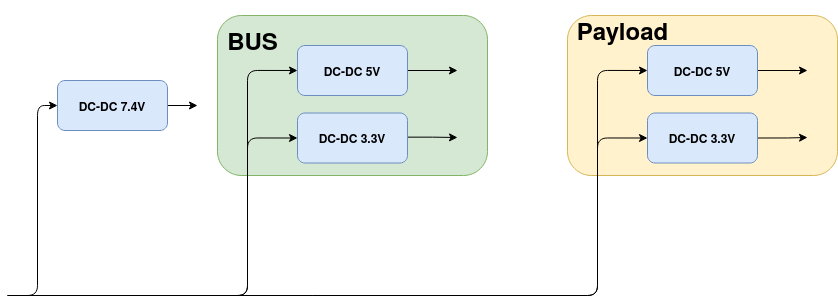
\includegraphics[scale=0.4]{dcdc.png}
   	\caption{Power processing}
   	\label{fig: ltc4015}
   \end{figure}
  
  One of important tasks of the EPS and PPU is to deploy 2 UHF antennas. To accomplish this task and provide a battery voltage to deployment mechanism, used 2 power lines for each UHF antenna with two TPS1H200A load switches in series for each line. To activate antenna release, two signals must be send from the microcontroller which enable the load switch to commutate and provide a power to accomplish antenna release on the Fig.\ref{fig: PPU} antenna release mechanism shown as ARM1 and ARM2. 
  
  In addition, PPU provide a current and voltage sensing of 16 analog lines,  which get converted via ADC MAX1231 that provide an SPI signal. 
  
  Figure \ref{fig: PPU} Illustrate the simple PPU architecture block diagram. 
  
  \begin{figure}[h]
  	\centering
  	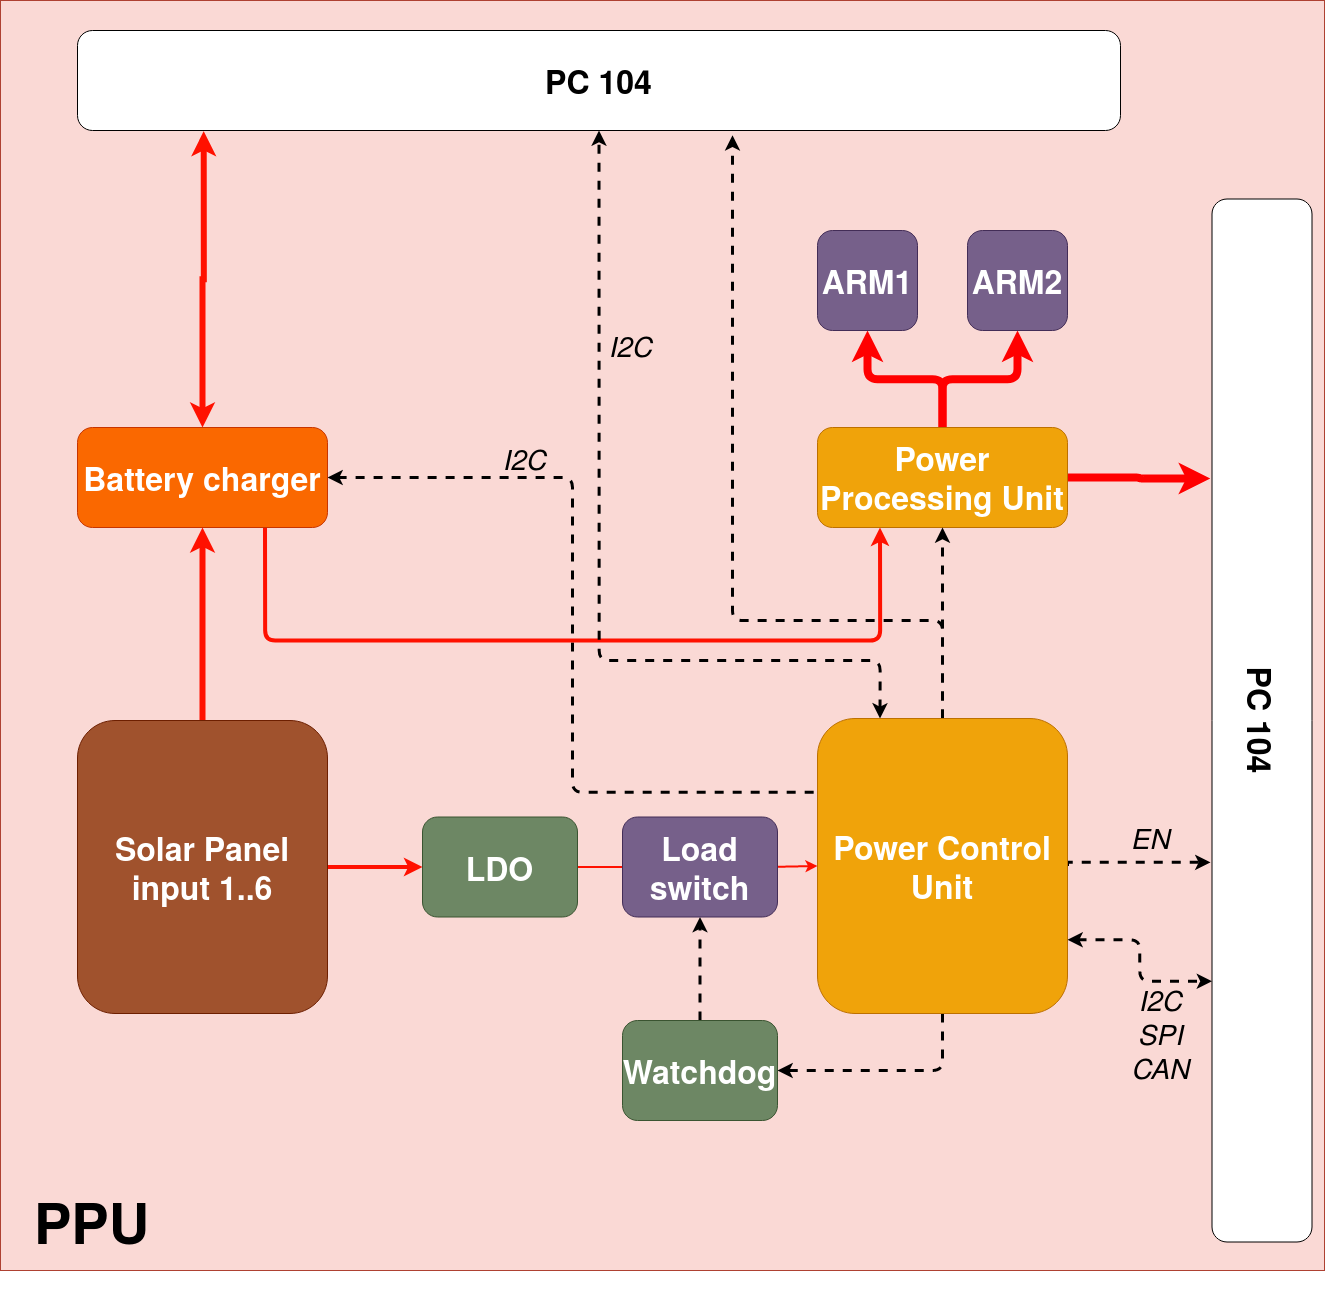
\includegraphics[scale=0.3]{PPU.png}
  	\caption{Power Processing Unit}
  	\label{fig: PPU}
  \end{figure}
  
     \subsection{Battery Pack}
  
 Battery pack board used to provide a power storage for the EPS by using of 4 li-ion batteries with a 2 series 2 parallel configuration. One of the EPS requirements is to provide capacity of 160 Wh which can be made by using 2 battery packs with LI-ion batteries samsung INR21700 with a capacity of 4900mAh.
 
 \begin{figure}[h]
 	\centering
 	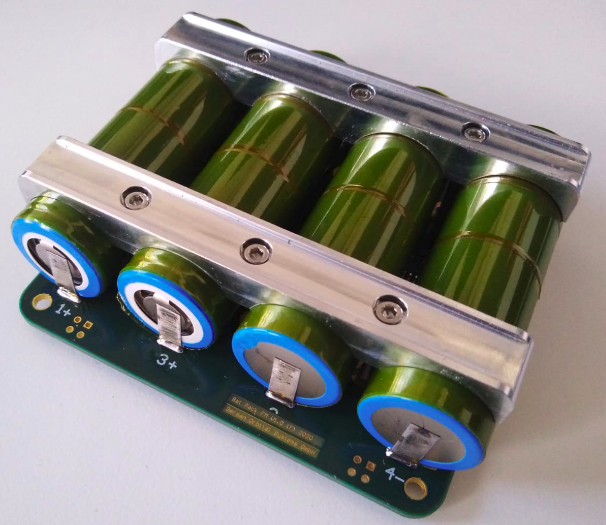
\includegraphics[scale=0.37]{bat.png}
 	\caption{Battery pack board}
 	\label{fig: bat}
 \end{figure}
 
  As was discussed in the background section \ref{sec:tech1} Li-ion batteries required a protection circuit to prevent overcharge, over-discharge and a fast discharge(short). For the battery pack board every two cells in the series have their own protection integrated chip BQ29700D which has an overcharge, over-discharge and short protection. Due to 2S2P configuration, batteries which located in parallel have to be balance. BQ29209 is a battery balancer from Texas Instruments which \cite{23}"performs automatic cell-balance correction where the two cells are automatically corrected for voltage imbalance by loading the cell with the higher voltage with a small balancing current."  
  
  \begin{figure}[h]
  	\centering
  	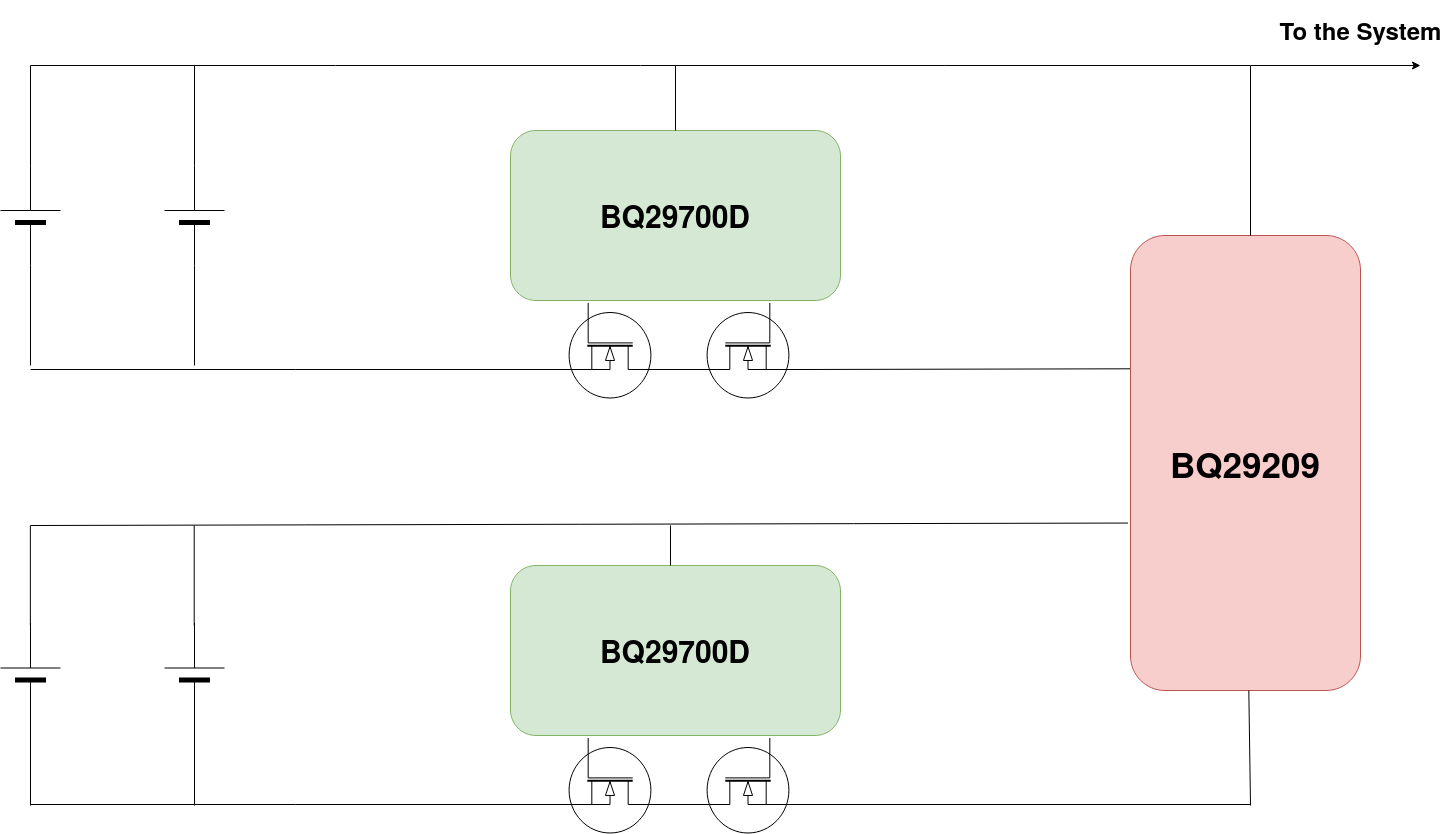
\includegraphics[scale=0.2]{2s2pMasterarbeit.png}
  	\caption{Battery protection-balancing}
  	\label{fig: Bat_prot_bal}
  \end{figure}
  
  The configuration \ref{fig: Bat_prot_bal} allows batteries to provide and collect the power at the same time keeping cells balanced and safe.
  
  Due to the space environment, temperature of the batteries can decrease bellow the temperature threshold. To avoid the battery temperature drop bellow the limit, was decided to use resistor heaters. Battery pack board has 2 temperature sensors that located under the batteries, which allow to measure the temperature close to the temperature of the batteries. The temperature sensors provide an I$^{2}$C to the PC104 connector that transfer the data signal to the microcontroller of the PPU. Microcontroller reads the signal and decide whether it need to provide a heat to the batteries or not. Heat is implemented by sending a enable signal from the microcontroller to the load switch TPS1H200A that has a function to transfer a power from the batteries to the low value resisters.  \\ \\ \\ \\
  
  
  \begin{figure}[h]
  	\centering
  	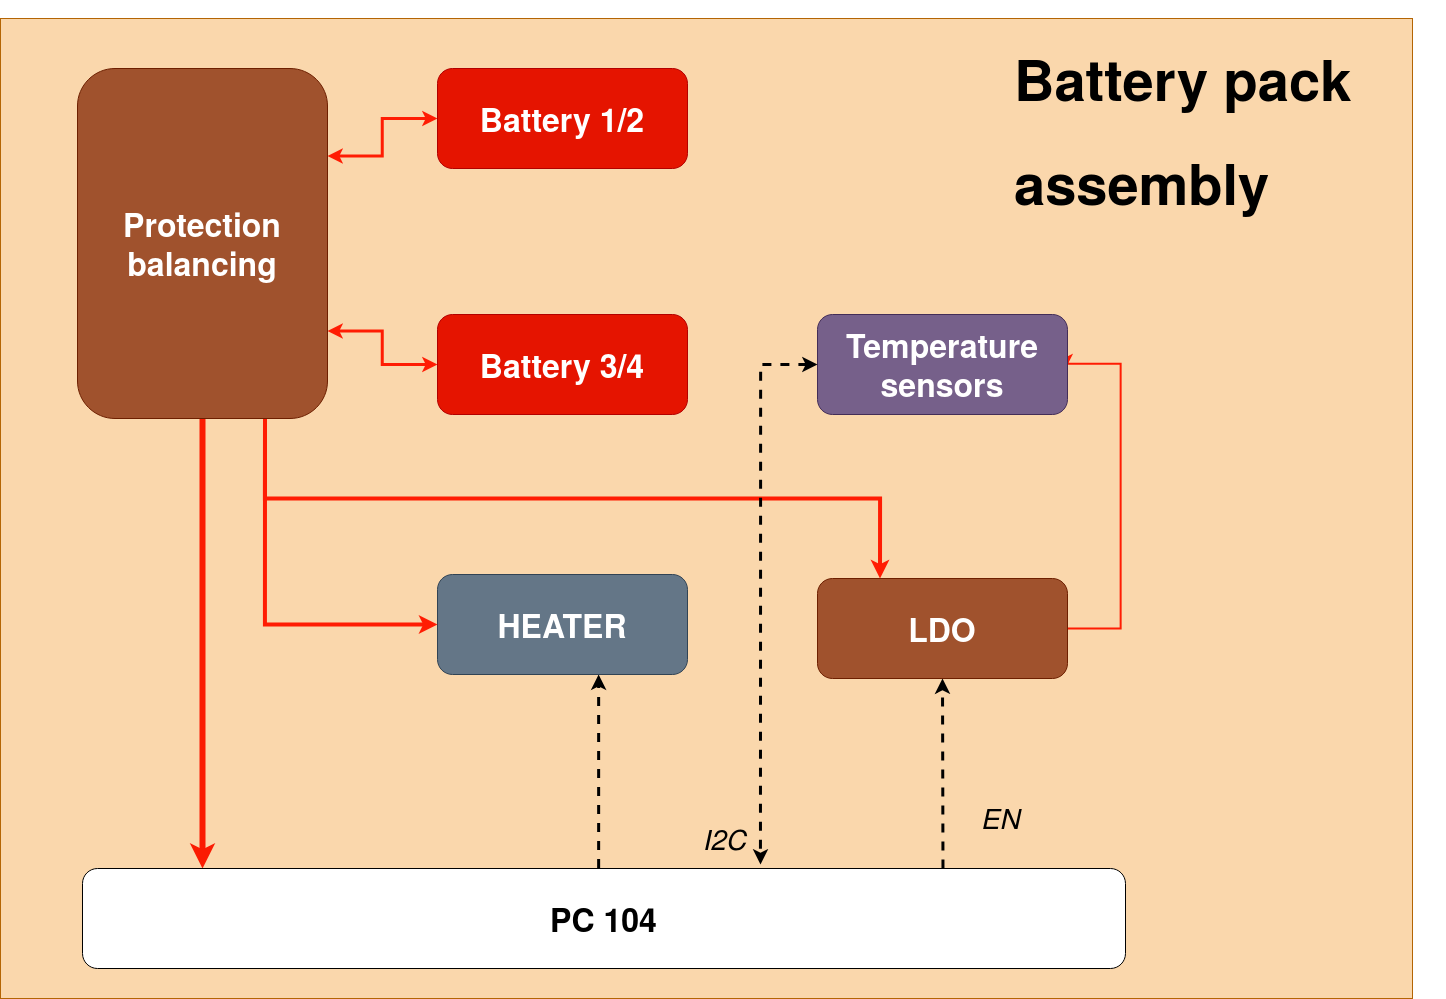
\includegraphics[scale=0.3]{BP.png}
  	\caption{Battery pack board}
  	\label{fig: BP}
  \end{figure} 
   
  
  \subsection{Power Distribution Unit}
  PDU is a part of the EPS that responsible for a power distribution and power monitoring. The main feature of PDU is the flexibility, that allows the PDU to fit every power requirement of the subsystem or payload.     To provide a power to the subsystems and payloads PDU uses 23 load switches of 3 different types TPS203x, TPS1H200A and FPF2701. The power distribution is controlled via EPS microcontroller by providing an enable signal to the pinhead connectors and partly by transmitting an I$^2$C signal to shift register that spread an array signal into the switches. 
  
  In order to measure a current of the power lines to observe a power consumptions of the subsystems and payloads, MAX4372 is used. Current sensors located one for each power line, which allows to measure the current of each line. MAX4372 has an analog output, which requires to use an ADC converter to convert an analog into a digital signal. To convert analog into a digital signal was decided to use MAX1231 ADC converter that provides an SPI output signal to the EPS microcontroller. 
  
    
  The detailed review, calculations and all explanations of the PDU board will be given in chapter \ref{sec:tech77}
  
    
  
    

    
  

  
  
  

